\documentclass[a4paper, 12pt, oneside, twocolumn]{article}
\usepackage[T1]{fontenc}
\usepackage{aurical}
\usepackage{csquotes}
\usepackage{booktabs}
\usepackage{textalpha}
\usepackage{url}
\usepackage{graphicx}
\setlength{\emergencystretch}{15pt}
\graphicspath{ {./figures/} }
\usepackage[figurename=]{caption}
\usepackage{fancyhdr}
\usepackage{amssymb}
\usepackage{array}
\usepackage{float}
\usepackage{imakeidx}
\usepackage{qtree}
\usepackage{microtype}
\usepackage[titles]{tocloft}
\usepackage{sectsty}
\usepackage[dvipsnames]{xcolor}
\usepackage{eso-pic,graphicx}
\usepackage[top=38mm, bottom=35mm, outer=23mm, inner=23mm]{geometry}
\setlength{\columnsep}{100pt}

\definecolor{customColor}{RGB}{40, 1, 55}

\usepackage{setspace}
\onehalfspacing

\renewcommand{\listfigurename}{List of Plates}
\makeindex[columns=2, title=Alphabetical Index, intoc]
% change color of text, example replace all \color{Goldenrod} with \color{lightgray}

\makeatletter % change only the display of \thepage, but not \thepage itself:
%\patchcmd{\ps@plain}{\thepage}{\color{customColor}{\thepage}}{}{}
\makeatother

\color{customColor}

\begin{document}
\Fontauri
\renewcommand\thefootnote{\color{customColor}\Fontauri{\arabic{footnote}}}
\let\oldfootnote\footnote
    \renewcommand{\footnote}[1]{\oldfootnote{\color{customColor}\Fontauri#1}}
\AddToShipoutPictureBG*{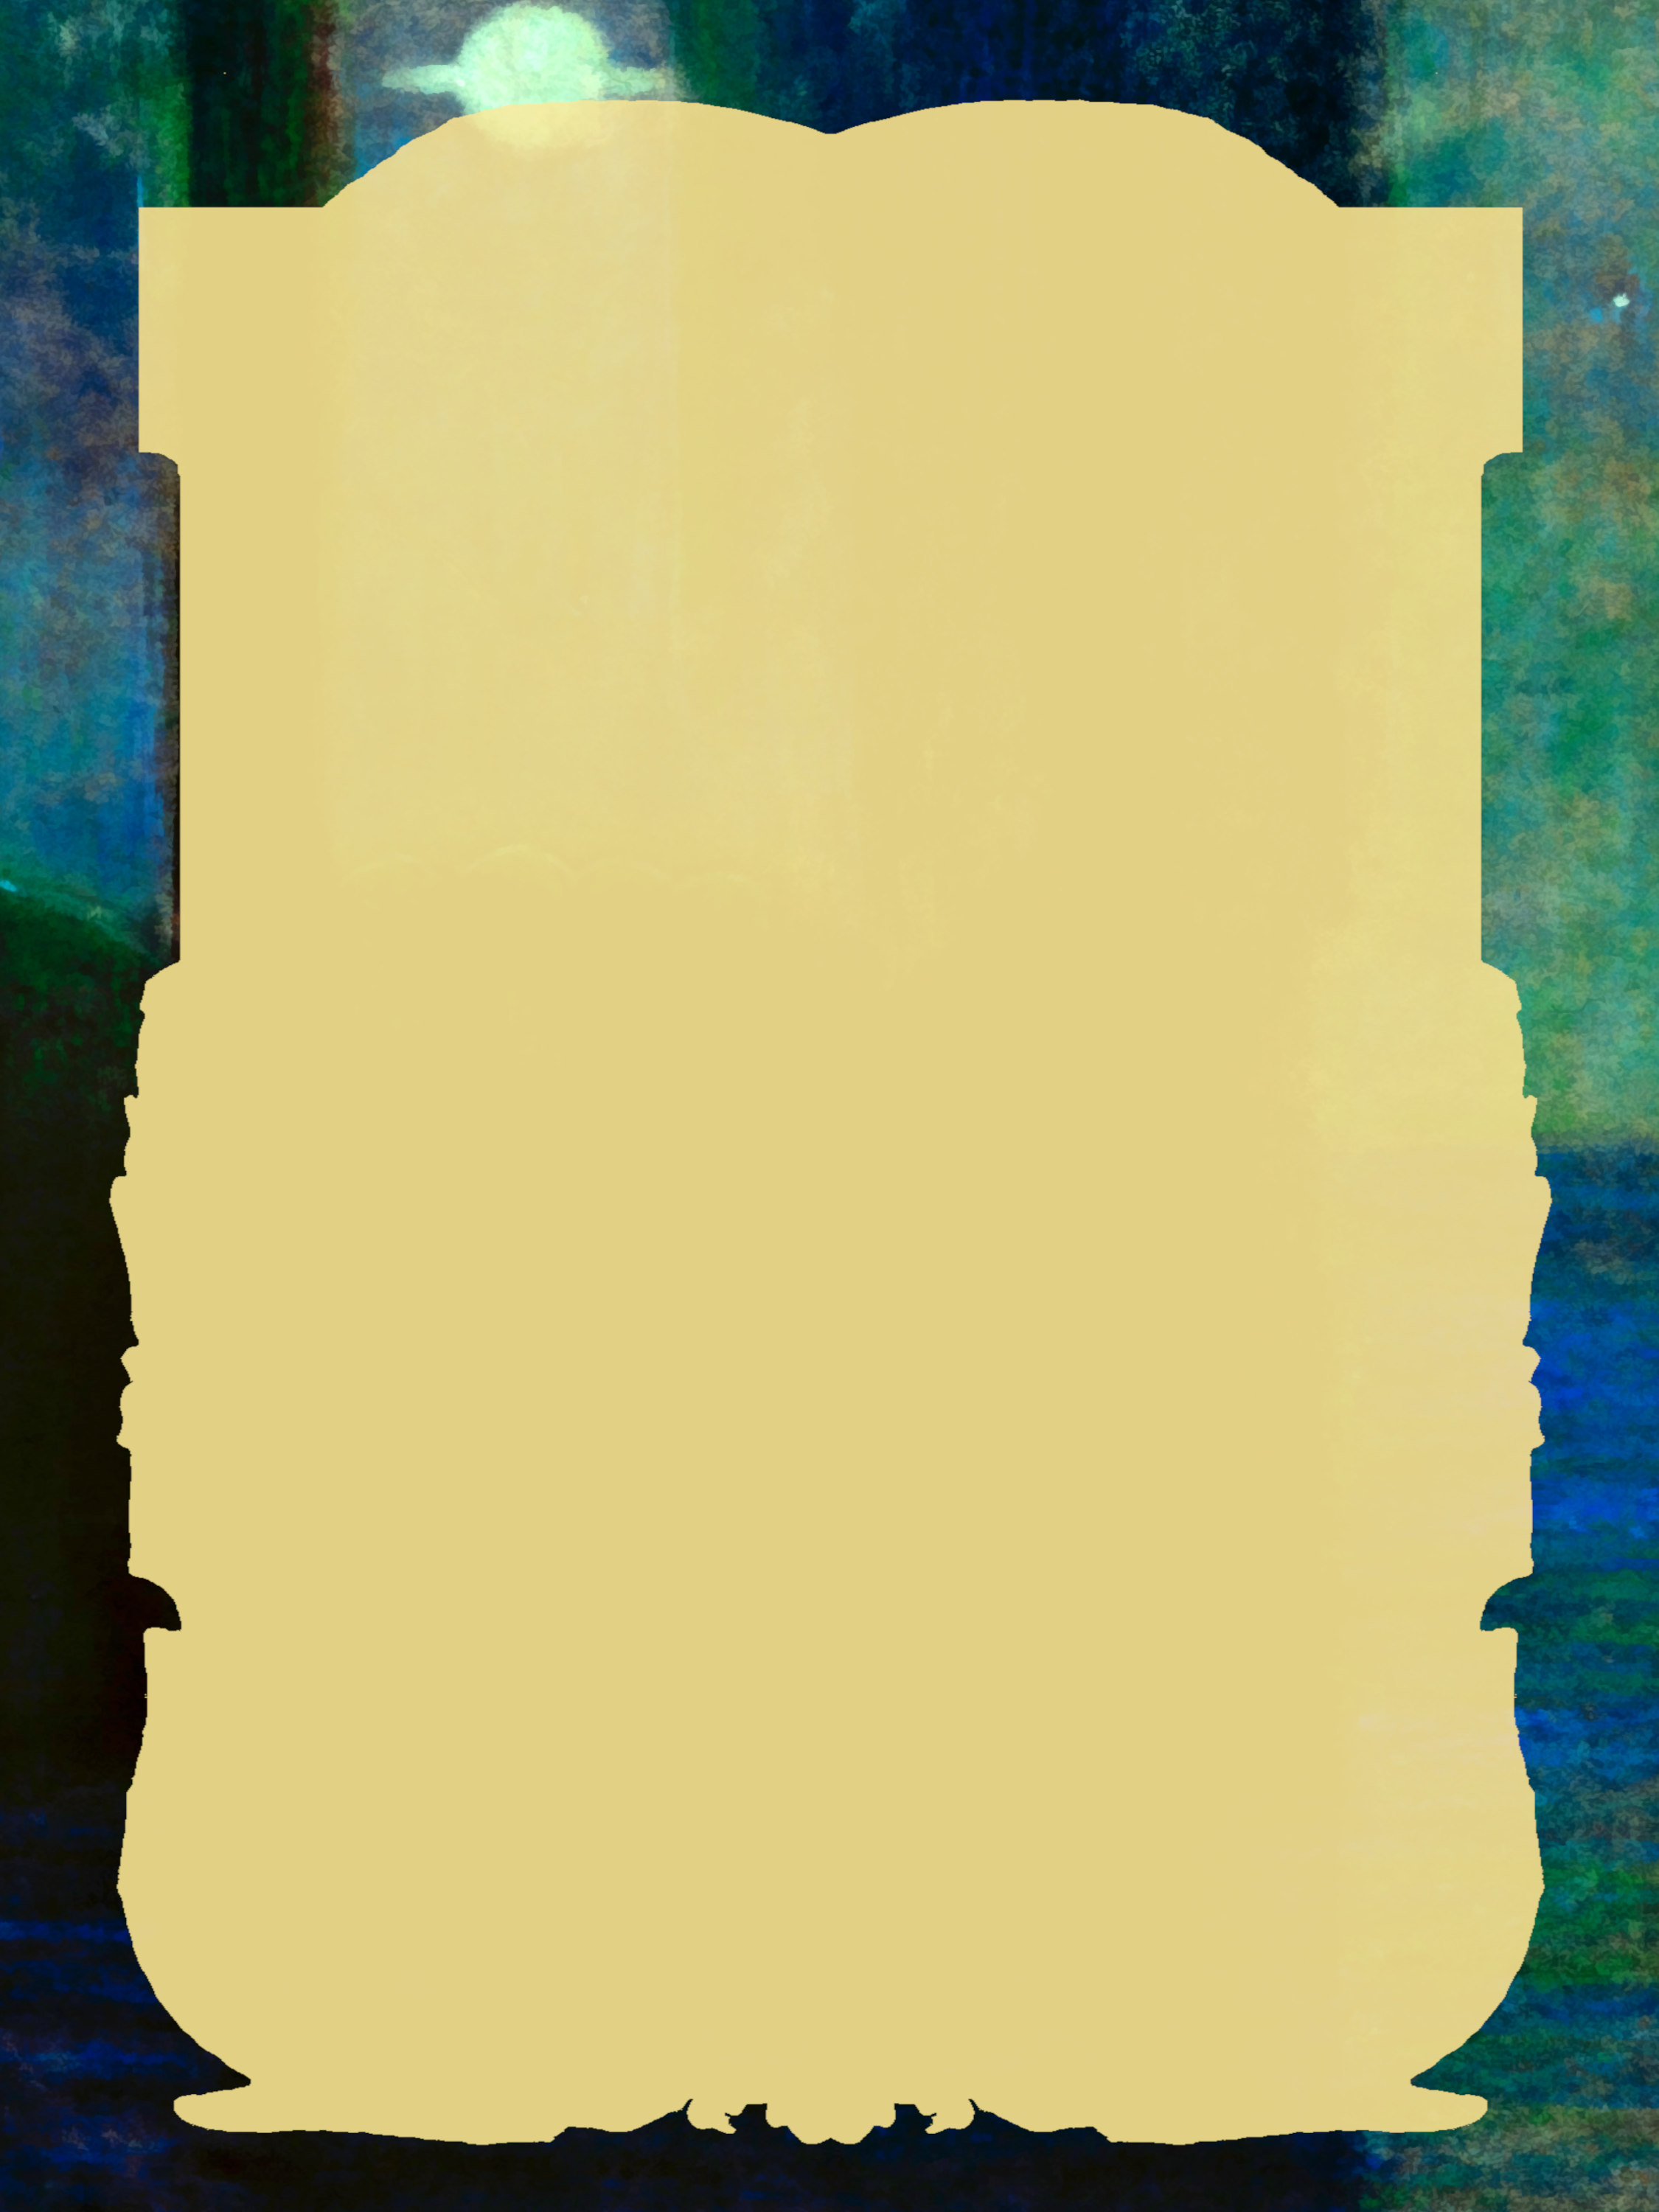
\includegraphics[width=\paperwidth,height=\paperheight]{night2.jpeg}}
\onecolumn
\begin{titlepage} % Suppresses headers and footers on the title page
	\centering % Centre everything on the title page
	\scshape % Use small caps for all text on the title page

	%------------------------------------------------
	%	Title
	%------------------------------------------------
	
	\rule{\textwidth}{1.6pt}\vspace*{-\baselineskip}\vspace*{2pt} % Thick horizontal rule
	\rule{\textwidth}{0.4pt} % Thin horizontal rule
	
	\vspace{0.75\baselineskip} % Whitespace above the title

        {\LARGE Remarks concerning Stones\\ said to have fallen from the Clouds,\\ both in these Days,\\ and in Ancient Times. \\} % Title
	
	\vspace{0.75\baselineskip} % Whitespace below the title
	
	\rule{\textwidth}{0.4pt}\vspace*{-\baselineskip}\vspace{3.2pt} % Thin horizontal rule
	\rule{\textwidth}{1.6pt} % Thick horizontal rule
	
	\vspace{1\baselineskip} % Whitespace after the title block
	
	%------------------------------------------------
	%	Subtitle
	%------------------------------------------------
	
	{By \scshape\Large Edward King, Esq. FRS, and FAS.\\} % Subtitle or further description
	
	\vspace*{1\baselineskip} % Whitespace under the subtitle
	
	%------------------------------------------------
	%	Editor(s)
	%------------------------------------------------
	
	\vspace{1\baselineskip} % Whitespace before the editors

    %------------------------------------------------
	%	Cover photo
	%------------------------------------------------
	
\pagestyle{fancy}	%\includegraphics[scale=1]{cover}
	
	%------------------------------------------------
	%	Publisher
	%------------------------------------------------
		
	\vspace*{\fill}% Whitespace under the publisher logo
	
	London 1796 % Publication year
	
	{\small G. Nicol, Bookseller to His Majesty, Pall-Mall. } % Publisher

	\vspace{1\baselineskip} % Whitespace under the publisher logo

    Internet Archive Online Edition  % Publication year
	
	{\small Attribution NonCommercial ShareAlike 4.0 International } % Publisher
\end{titlepage}
\AddToShipoutPictureBG*{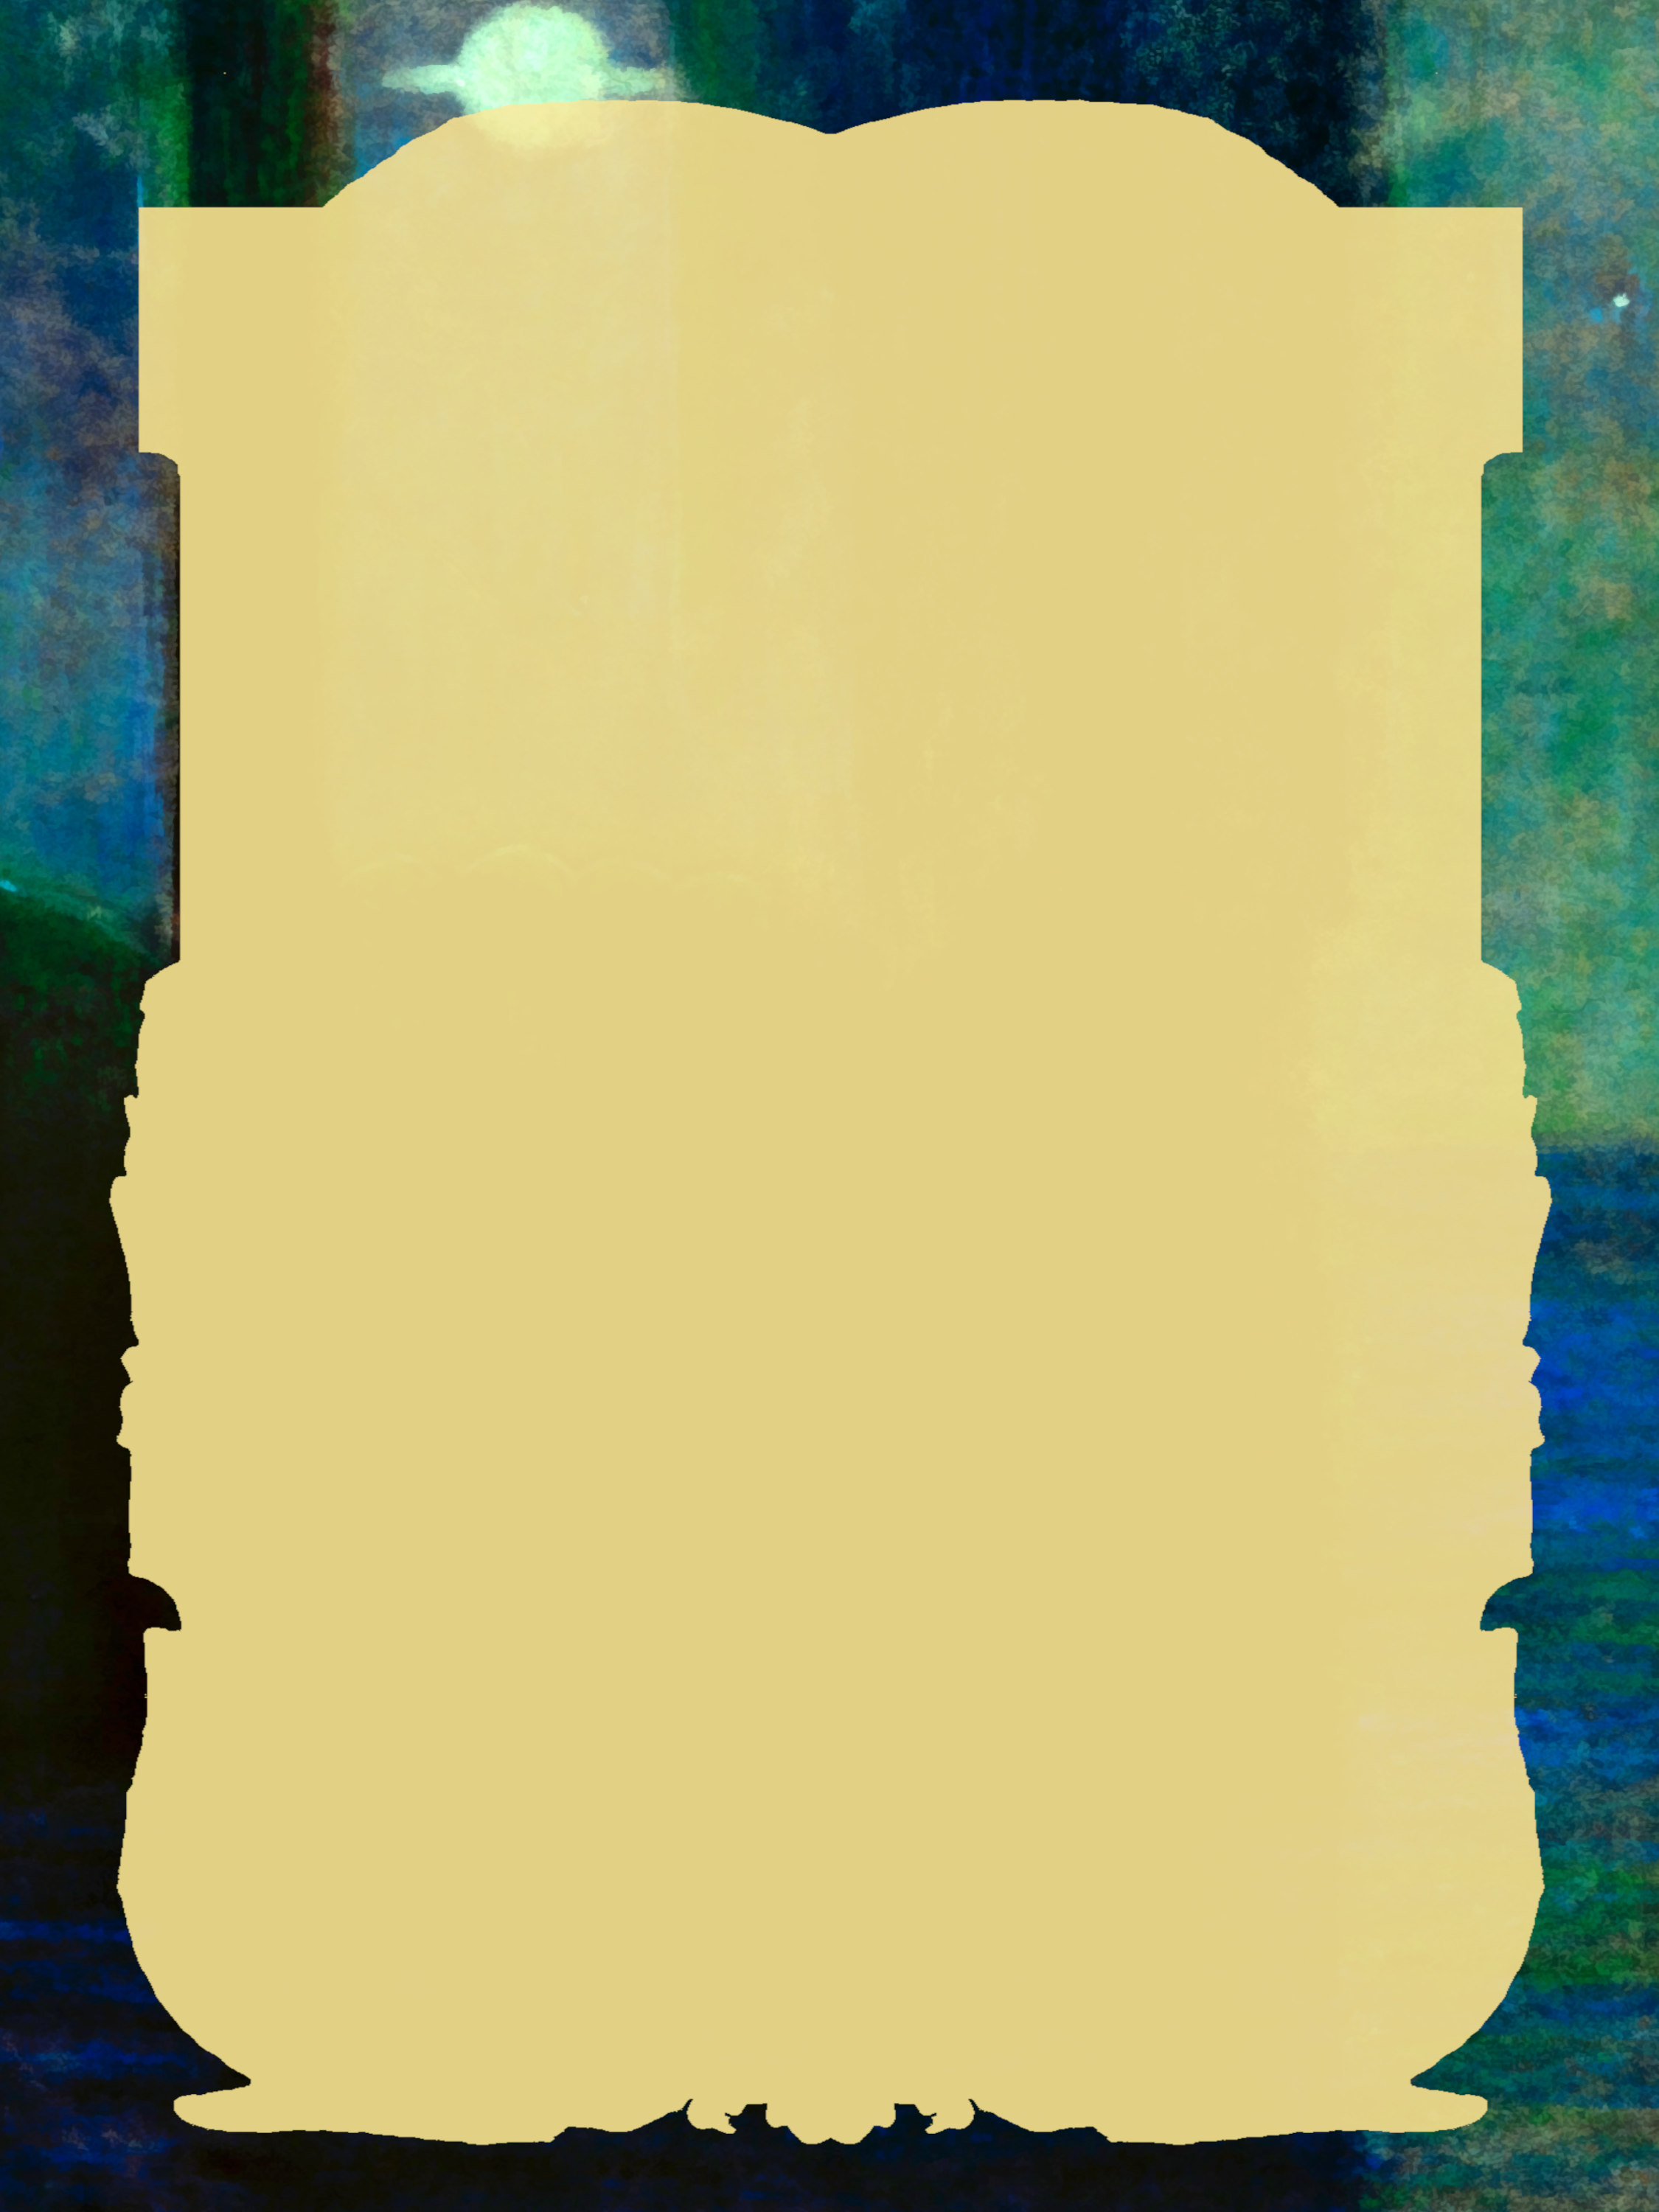
\includegraphics[width=\paperwidth,height=\paperheight]{night2.jpeg}}
\pagestyle{fancy}
\fancyhf{} % clear all header and footers
\renewcommand{\headrulewidth}{0pt} % remove the header rule
\cfoot{\Fontauri{\thepage}}
\vspace*{\fill}
\begin{quote} 
``Res ubi plurimum proficere, et valere possunt, collocari debent.''

--- \emph{Cicero de Orat. 37.}
\end{quote}
\vspace*{\fill}
\clearpage
\pagestyle{fancy}
\fancyhf{} % clear all header and footers
\renewcommand{\headrulewidth}{0pt} % remove the header rule
\rfoot{\Fontauri{\thepage}}
\twocolumn
\AddToShipoutPictureBG{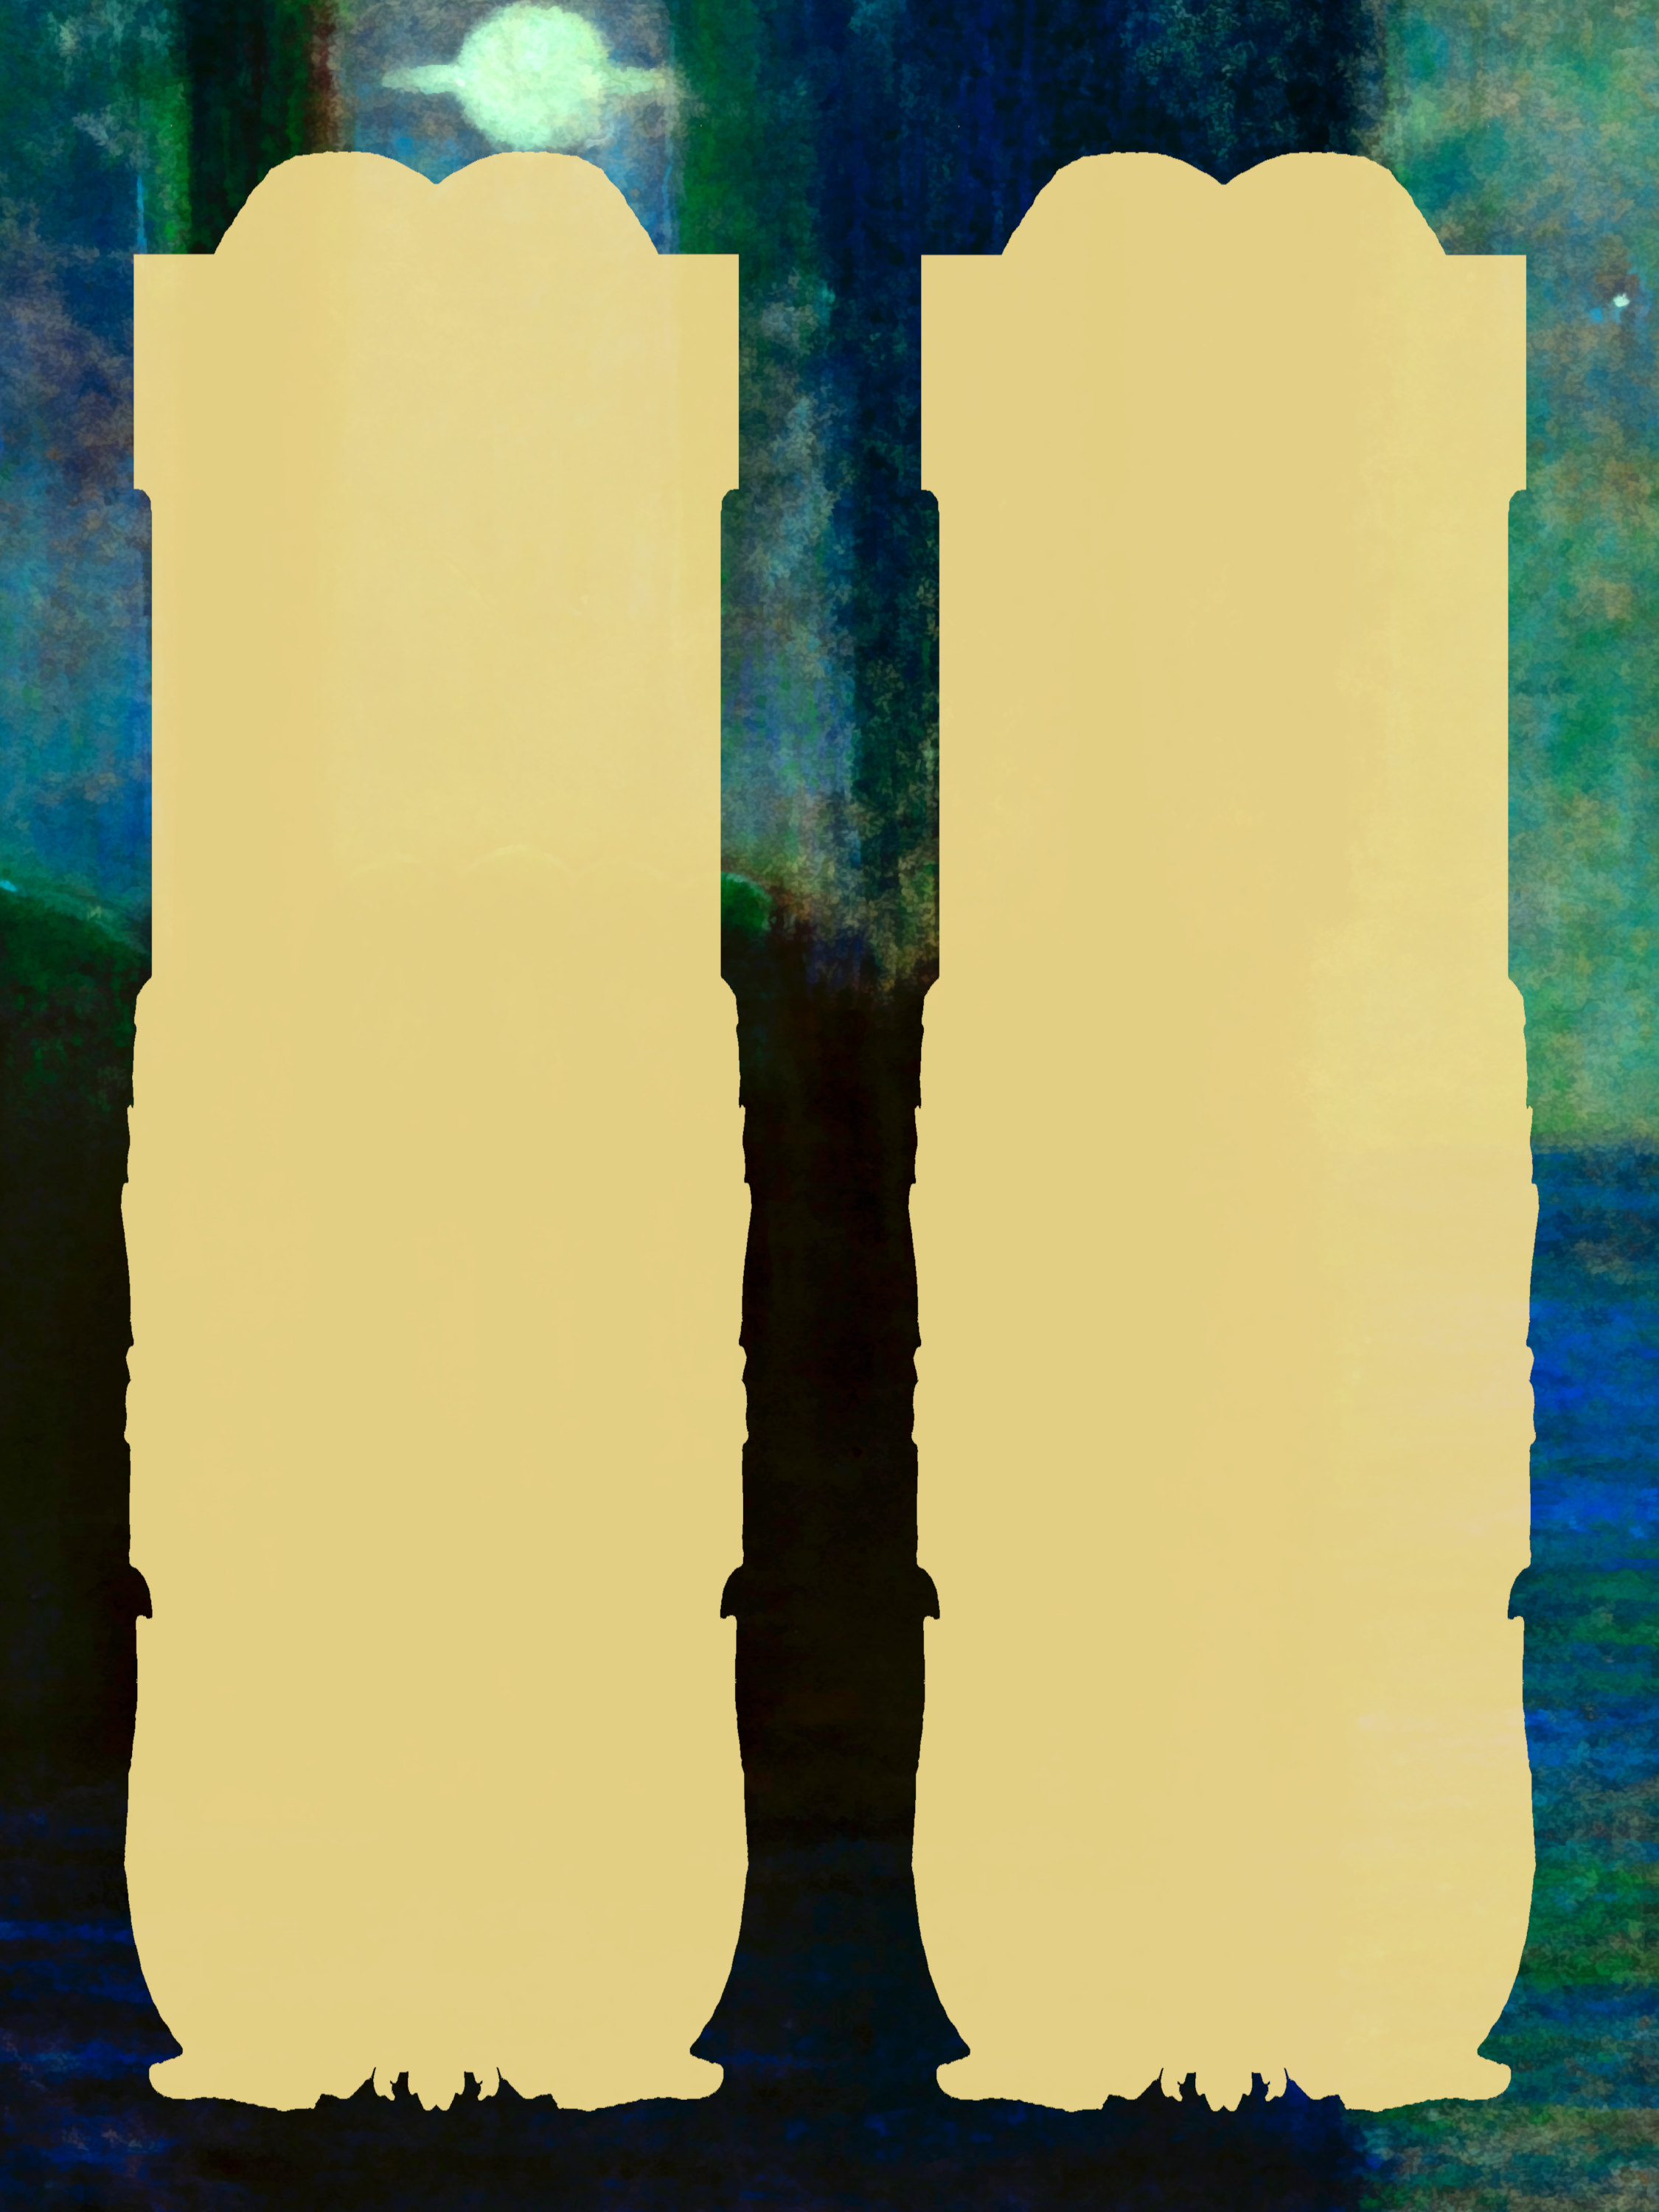
\includegraphics[width=\paperwidth,height=\paperheight]{night1.jpeg}}
\setlength{\parskip}{1mm plus1mm minus1mm}
\setcounter{tocdepth}{3}
\setcounter{secnumdepth}{3}
\paragraph{}
Having received this last winter, from Sir Charles Blagden, some very curious \emph{manuscript} accounts, concerning a surprising shower of stones; which is said, on the testimony of several persons, to have fallen in Tuscany, on the 16\textsuperscript{th} of June, 1794; --- and having also perused, with much attention, a very interesting pamphlet, written in Italian, by \emph{Abbate Ambrose Soldani}, Professor of mathematics, in the University of Siena, containing an extraordinary and full detail of such facts as could be collected relating to this shower; the whole has appeared to me to afford such an ample field for philosophical contemplation, and also for the illustration of ancient historic facts; that (leaving the whole to rest upon such testimony as the learned Professor has already collected together; and to be supported by such further corroboration, as I am informed is likely \emph{soon} to arrive in England,) I cannot but think it doing some service to the cause of literature, and science, to give to the world, in the earliest instance, a short abridgement of the substance of the whole of the information; expressed in the most concise and plainest language, in which it is possible for me to convey a full and exact idea of the phenomenon.

It may be of some use, and afford satisfaction to several curious persons, to find the whole here compressed in so small a compass.

And, as I shall add my own conclusions without reserve; because the whole of the phenomenon tends greatly to confirm some ideas which I had previously been led to form, many years ago, concerning the consolidation of certain species of stone; it may open a door for further curious investigation.

And it may at least amuse, if not instruct; whilst I add a short detail of uncommon facts, recorded in ancient history, and tending to show clearly, that we are not without precedents of \emph{similar events} having happened, in the early ages of antiquity.

On the 16\textsuperscript{th} of June, 1794, a tremendous cloud was seen in Tuscany, near Siena, and Radacofani; coming from the north, about seven o'clock in the evening; --- sending forth sparks, like rockets; --- throwing out smoke like a furnace; --- rendering violent explosions, and blasts, more like those of cannon, and of numerous muskets, than like thunder; --- and casting down to the ground hot stones: --- whilst the lightning that issued from the cloud was remarkably red; and moved with \emph{less} velocity than usual.

The cloud appeared of different shapes; to persons in different situations; and remained suspended a long time: but everywhere was plainly seen to be burning, and smoking like a furnace.

And its original height, from a variety of circumstances put together, seems to have been much above the common region of the clouds.

The testimony, concerning the falling of the stones from it, appears to be almost unquestionable: --- and is, evidently, from different persons, who had no communication with each other.

For first; the fall of four stones is precisely ascertained: one of which was of an irregular figure, with a point like that of a diamond; --- weighed five pounds and an half; --- and had a vitriolic smell. --- And another weighed three pounds and an half; --- was black on the outside, as if from smoke; --- and, internally, seemed composed of matter of the colour of ashes; --- in which were perceived small spots of metals, of gold and silver.

And, besides these, Professor Soldani of Siena, was shown about fifteen others: the surfaces of which were glazed black, like a sort of varnish; --- resisted acids; --- and were too hard to be scratched with the point of a penknife.

Signior \emph{Andrew Montauli}, who saw the cloud, as he was travelling, described it as appearing much above the common region of the clouds; and as being clearly discerned to be on fire; --- and becoming white, by degrees; not only where it had a communication, by a sort of stream of smoke and lightning, with a neighbouring similar cloud: but also, at last, in two-third parts of its whole mass, which was originally black. And yet he took notice, that it was not affected by the rays of the sun, though they shone full on its lower parts. --- And he could discern as it were the bason of a fiery furnace, in the cloud, having a whirling motion.

This curious observer gives an account also, of a stone, which he was assured fell from the cloud, at the feet of a farmer; and was dug out of the ground, into which it had penetrated. --- And he says, that it was about five inches long, and four broad; nearly square; and polished: black on the surface, as if smoked; but within, like a sort of sand-stone, with various small particles of iron, and bright metallic stars.

Other stones are described by him; which were said to have fallen at the same time: were triangular; and terminated in a sort of (pyramidal) or conical figure. --- And others were so small as to weigh not more than an ounce.

Professor Soldani saw another stone, said to have fallen from the cloud, which had the figure of a parallelopiped, blunted at the angles; and was as it were varnished, on the outside, with a black crust; and quite unlike any stones whatever of the soil of the country where it had fallen.

Two ladies being at \emph{Cozone}, about 20 miles from \emph{Siena}, saw a number of stones fall, with a great noise, in a neighbouring meadow: one of which, being soon after taken up by a young woman, burnt her hand: another burnt a countryman's hat: and a third was said to strike off the branch of a mulberry tree; and to cause the tree to wither.

Another stone, of about two ounces weight, fell near a girl watching sheep; a young person, whose veracity it is said could not be doubted. --- This stone, the Professor tells us, is also a parallelopiped, with the angles rounded; and its internal substance is like that of the others; only with more metallic spots; especially when viewed with a magnifying glass: and the black external crust appears to be minutely crystallized.

Many others, of a similar kind, were in the possession of different persons at Siena.

And besides the falling of these from the cloud, there is described to have been a fall of sand; seen by keepers of cattle near \emph{Cozone}, together with the falling of what appeared like squibs; and which proved afterwards to be stones, of the sort just described, weighing two or three ounces: --- and some only a quarter of an ounce.

Amongst other stones that fell; was one weighing two pounds, and two ounces; which was also an oblong parallelopiped, with blunted angles, (as they are called, but which I think meant plainly prismatic terminations, and are said to have been about an inch in height;) and this was most remarkable for having, a small circle, or sort of belt round it, in one part; wherein the black crust appeared more smooth; and shining like glass; as if that part had suffered a greater degree of heat than the rest.

Another, also, was no less remarkable, for having many rounded cavities on its surface: as if the stone had been struck with small balls, whilst it was forming; and before it was hardened; which left their impressions. --- And some appearances, of the same kind, were found on one of the four surfaces of another stone, in the possession of Soldani.

On minute examination, the Professor found the stones were composed of blackish \emph{crystals}, of different kinds; with metallic or pyritic spots, all united together by a kind of consolidated ashes. --- And, on polishing them, they appeared to have a ground of a dark ash colour; intermixed with cubical blackish crystals, and shining pyritic specks, of a silver and gold colour.

The conclusion which Professor Soldani evidently forms, is; \emph{that the stones were generated in the air, by a combination of mineral substances, which had risen somewhere or other}, \textbf{as exhalations}, \emph{from the earth}: but, as he seems to think, \emph{not from} Vesuvius.

The names of many persons, besides those already referred to, are mentioned; who were eye witnesses to the fall of the stones. And several \emph{depositions} were made, \emph{in a regular juridical manner}, to ascertain the truth of the facts.

The space of ground, within which the stones fell, was from three to four miles.

The falling of them, was \emph{the very day after} the great eruption of Vesuvius.

And the distance of the place, from Vesuvius, could not be less than two hundred miles, and seems to have been more.

Vesuvius is situated \emph{to the south} of the spot: and the cloud came \emph{from the north}; about thirteen, or at most eighteen hours, after the eruption.

Now, putting all these circumstances together, I cannot but venture to form a conclusion, somewhat different from Professor Soldani's; though perfectly agreeing with his general principles.

From a course of observations, and inquiries, which I have been led to pursue, for a great many years: tending to elucidate the history of extraneous fossils, and of the deluge; I have long been convinced, that stones in general, and strata of rocks, of all kinds, have been formed by \emph{two} very different operations of those elements, which the wisdom, and omnipotent hand of God, has ordained, and created.

The one, by means of fire: --- and the other, by means of water.

And, of each sort, there are two subdivisions.

Of the stones, and rocks, formed by fire; --- there are some, (besides lavas,) whose component parts, having been previously fused, and in a melted state, did merely cool, and harden \emph{gradually}.

And there are others; whose component parts, having been fused, and in a melted state, and having so become completely liquid; did instantly, by the operation of the powers of \emph{attraction}, become crystallized.

And, in like manner; of stones, and of strata of rocks, formed by means of water; --- there are some, which having had their component parts brought together, in a fluid state; did then merely become gradually settled; and by the power of attraction, and the mixture of crystalline particles, were hardened by degrees.

And there are others: which, having had their component parts, in like manner, brought together by water, did yet, on account of the peculiar nature, and more powerful \emph{attraction} of those parts, \emph{instantly} crystallize.

And both of stones, and of strata of rocks, formed by fire; and of stones, and of strata of rocks formed by means of water; there are some such, as have been slowly consolidated by the first kind of operation; namely by the gradual cooling or settling of the substances; which yet do contain imbedded in them, crystals formed by the latter kind of operation.

Instances of which, we seem to have, in some granites, on the one hand; --- and in some sorts of limestones on the other.

To this I must add also; that there appear further, to have been some stones formed \emph{by a sort of precipitation}: much in the same manner as \emph{Grew} describes\footnote{\Fontauri{In his Anatomy of Plants, p. 41-184.}} the kernels, and stones of fruit to have been hardened.

And I have met with many instances, wherein it appears unquestionably, that all these kind of processes in nature are going on continually: and that extraneous substances are actually enclosed, and \emph{continually inclosing}, which could not be \emph{antediluvian}; but must have been \emph{recent}.

To these short premises, I must beg leave to add; that in two papers formerly printed in the Philosophical Transactions,\footnote{\Fontauri{Vol. 63. p. 241 --- and Vol. 69. p. 35.}} I endeavoured, by some very remarkable instances, to prove, that iron, wherever it comes into combination with any substances that are tending to consolidation, \emph{hastens the process exceedingly}; --- and also renders the hardness of the body much greater.

And I have also endeavoured, elsewhere,\footnote{\Fontauri{In the Morsels of Criticism, p. 103.}} to show, in consequence of conclusions deduced from experiments of the most unquestionable authority, that \emph{air}, in its various shapes and modifications, is indeed \emph{itself} the great consolidating fluid, out of which solid bodies are composed; and by means of which the various attractions take place, which form all the hard bodies, and visible substances upon earth.

From all these premises then, it was impossible for me not to be led to conclude; that we have, in this august phenomenon of the fall of stones from the clouds, in Tuscany, an obvious proof, as it were before our eyes, of the combined operation of those very powers, and processes, to which I have been alluding.

It is well known; that pyrites, which are composed of iron, and sulphur, and other adventitious matter, when laid in heaps, and moistened, will take fire.

It is also well known, that a mixture of pyrites of almost any kind, beaten small, and mixed with iron filings and water, when buried in the ground will take fire; and produce a sort of artificial volcano. And, surely then, wherever a vast quantity of such kind of matter should at any time become mixed together, as flying dust, or ashes; and be by any means condensed together, or compressed, the same effect might be produced, even in the atmosphere and air.

Instead, therefore, of having recourse to the supposition, of the cloud in Tuscany having been produced by any other kind of exhalations from the earth; we may venture to believe, that an immense cloud of ashes, mixed with pyritic dust, and with numerous particles of iron, having been projected from Vesuvius to a most prodigious height, became afterwards condensed in its descent; --- took fire, both of itself, as well as by means of the electric fluid it contained; --- produced many explosions; --- melted the pyritic, and metallic, and argillaceous particles, of which the ashes were composed; --- and, by this means, had a sudden crystallization, and consolidation of those particles taken place, which formed the stones of various sizes, that fell to the ground: \emph{but did not harden the clayey ashes so rapidly as the metallic particles crystallized}; and, therefore, gave an opportunity for \emph{impressions to be made} on the surfaces of some of the stones, as they fell, by means of the impinging of the others.

Nor does it appear to me, to be any solid objection to this conclusion, either that Vesuvius was so far distant; or that the cloud came from the north.

For, if we examine Sir William Hamilton's account of the very eruption in question,\footnote{\Fontauri{In the Philos. Trans. for 1795, p. 91, 92.}} we shall find, that he had reason to conclude, that the \emph{pine-like} cloud of ashes projected from Vesuvius, at one part of the time during this eruption, was twenty-five or thirty miles in height; and, if to this conclusion we add, not only that some ashes actually were carried to a greater distance than \emph{two hundred miles}\footnote{\Fontauri{This is mentioned by Sir William Hamilton himself, p. 105.}}; but that, when any substance is at a vast height in the atmosphere, a very small variation of the direction of its course, causes a most prodigious variation in the extent of the range of ground where it shall fall; (just as the least variation in the angle, at the vertex of an \emph{isosceles} triangle, causes a very great alteration in the extent of its base;) we may easily perceive, not only the possibility, but the probability, that the ashes in question, projected to so vast an height, were first carried even beyond \emph{Siena} in Tuscany, northward; and then brought back, by a contrary current of wind, in the direction in which they fell.

Sir William Hamilton himself formed somewhat this sort of conclusion, on receiving the first intimation of this shower of stones from the Earl of Bristol.\footnote{\Fontauri{See Philos. Trans. for 1795, p. 104, 105.}}

I cannot therefore but allow my own conclusion to carry conviction with it to my own mind; and to send it forth into the world; as a ground, at least, for speculation, and reflection, to the minds of others.

That ashes, and sand, and pyritic and sulphureous dust, mixed with metallic particles from volcanoes; fit for the instantaneous crystallization, and consolidation of such bodies as we have been describing, are often actually floating in the atmosphere, at incredible distances from volcanoes, and more frequently than the world are at all aware of, is manifest from several well attested facts.

On the 26\textsuperscript{th} of December, 1631, Captain \emph{Badily}, being in the Gulf of Volo, in the Archipelago, riding at anchor, about ten o'clock at night, it began to rain \emph{sand} and \emph{ashes}; and continued to do so till two o'clock the next morning. The ashes lay about two inches thick on the deck: so that they cast them overboard just as they had done snow the day before. There was no wind stirring, when the ashes fell: and yet this extraordinary shower was not confined merely to the place where \emph{Badily's} ship was\footnote{\Fontauri{See Lowthorp's Abridgement of the Philos. Trans. Vol. 2. p. 143.}}; but, as it appeared afterwards, was extended so widely to other parts, that ships coming from \emph{St. John d'Acre} to that port, being at the distance of \emph{one hundred leagues} from thence, were covered with the same sort of ashes. And no possible account could be given of them, except that they might come from Vesuvius.

On the 23rd of October, 1755, a ship belonging to a merchant of Leith, bound for Charles Town, in Carolina, being betwixt Shetland and Iceland, and about twenty-five leagues distant from the former, and therefore about three hundred miles from the latter, a shower of dust fell in the night upon the decks.\footnote{\Fontauri{Philos. Trans. Vol. 49. p. 510.}}

In October, 1762, at \emph{Detroit}, in America, was a most surprising darkness, from day-break till four in the afternoon, during which time some rain falling, brought down, with the drops, sulphur and dirt; which rendered white paper black, and when burned fizzed like wet gunpowder:\footnote{\Fontauri{Philos. Trans. Vol. 53. p. 54.}} and whence such matter could originally be brought, appeared to be past all conjecture, unless it came so far off as from the volcano in Guadeloupe.

Condamine says, the ashes of the volcano of \emph{Sangay}, in South America, sometimes pass over the provinces of Maca, and Quito; and are even carried as far as Guayaquil.\footnote{\Fontauri{Condamine's Journal, p. 57.}}

And Hooke says,\footnote{\Fontauri{In his Experiments, p. 35.}} that on occasion of a great explosion from a volcano, in the island of Ternata, in the East Indies, there followed so great a darkness, that the inhabitants could not see each other the next day: and he justly leads us to infer what an immense quantity of ashes must, by this means, have been showered down somewhere on the sea; because at \emph{Mindanao}, an hundred miles off, all the land was covered with ashes a foot thick.

And now, I must add; that such kind of \emph{falling of stones from the clouds}, as has been described to have happened in Tuscany, seems to have happened also in very remote ages, of which we are not without sufficient testimony; and such as well deserves to be allowed and considered, on the present occasion; although the knowledge of the facts was, at first, in days of ignorance and gross darkness, soon perverted to the very worst purposes.

In the Acts of the holy Apostles, we read, that the chief magistrate, at \emph{Ephesus}, begun his harangue to the people, by saying, ``Ye men of Ephesus, \emph{what man is there that knoweth not how that the city of the Ephesians is a worshipper of the great goddess Diana, and of the} \textbf{image} \emph{which fell down from Jupiter}?'' (or rather, as the original Greek has it) ``\emph{of} \textbf{that} \emph{which fell down from Jupiter}?'' And the learned \emph{Greaves} leads us to conclude this image of Diana to have been nothing but \emph{a conical, or pyramidal stone}, that fell from the clouds. For he tells us,\footnote{\Fontauri{Pyramidographia, Vol. 1. 89-91.}} on unquestionable authorities, that many others of the images of heathen deities were merely such.

Herodian expressly declares,\footnote{\Fontauri{Lib. 5.}} that the Phoenicians had no statue of the sun, polished by hand, to express an image; but only had a certain \emph{great stone, circular below, and ending with a sharpness above, in the figure of a cone, of black colour. And they report it to have fallen from heaven, and to be the image of the sun}.

So Tacitus says,\footnote{\Fontauri{Lib. 2.}} that at Cyprus, \emph{the image of Venus was not of human shape; but a figure rising continually round, from a larger bottom to a small top, in conical fashion}. And it is to be remarked, that \emph{Maximus Tyrius} (who perhaps was a more accurate mathematician,) says, the stone was \emph{pyramidal}.

And in Corinth, we are told by \emph{Pausanias},\footnote{\Fontauri{In his Corinthiaca.}} that the images both of \emph{Jupiter Melichius}, and of \emph{Diana}, were made (if made at all by hand) with little or no art. The former being represented by a pyramid, the latter by a column.

\emph{Clemens Alexandrinus} was so well acquainted with these facts, that he even concludes\footnote{\Fontauri{Clem. Alex. lib. 1. --- Stromatum.}} the worship of such stones to have been the first, and earliest idolatry, in the world.

It is hard to conceive how mankind should ever have been led to so accursed an abomination, as the worship of stocks, and stones, at all: but, as far as anything so horrid is to be accounted for, there is no way so likely of rendering a possible account; as that of concluding, that some of these pyramidal stones, at least, like the image of \emph{Diana}, actually did fall, in the earliest ages, from the clouds; in the same manner as these pyramidal stones fell, in 1794, in Tuscany.

\emph{Plutarch}, it is well known, mentions\footnote{\Fontauri{In Vita Lysandri.}} a stone which formerly fell from the clouds, in \emph{Thrace}, and which \emph{Anaxagoras} fancied\footnote{\Fontauri{Diogenes in Anaxag.}} to have fallen from the sun.

And it is very remarkable, that the old writer, from whom Plutarch had his account, described the cloud, from which this stone was said to fall, in a manner (if we only make some allowance for a little exaggeration in barbarous ages,) very similar to \emph{Soldani's} account of the cloud in Tuscany. --- It hovered about for a long time; seemed to throw out splinters, which flew about, like wandering stars, before they fell; and at last it cast down to the earth a stone of extraordinary size.

Pliny,\footnote{\Fontauri{Historia Nat. lib. 2. cap. 59.}} who tells us that not only the remembrance of this event, but that the stone itself was preserved to his days, says, it was of a dark burnt colour. And though he does indeed speak of it as being of an extravagant weight and size, in which circumstance perhaps he was misled: yet he mentions \emph{another} of a moderate size, which fell in \emph{Abydos}, and was become an object of idolatrous worship in that place; as was still \emph{another}, of the same sort, at \emph{Potidæa}.

\emph{Livy}, who like \emph{Herodotus}, has been oftentimes censured as too credulous, and as a relater of falsehoods, for preserving traditions of \emph{an extraordinary kind}; which, after all, in ages of more enlarged information, have proved to have been founded in truth; describes\footnote{\Fontauri{Lib. 1. Sec. 31.}} a fall of stones to have happened on mount \emph{Alba}, during the reign of \emph{Tullus Hostilius}, (that is about 652 years before the Christian era), in words that exactly convey an idea of just such a phenomenon, as this which has so lately been observed in Tuscany.

He says, the senate were told, that \emph{lapidibus pluisse}, it had rained stones. And, when they doubted of the fact; and sent to inquire; they were assured that stones had actually fallen; and had fallen just as hail does, which is concreted in a storm.\footnote{\Fontauri{Haud aliter quam quum grandinem venti glomeratam in terras agunt, crebri cecidere cœlo lapides.}}

He mentions also shortly another shower of stones,\footnote{\Fontauri{Lib. 30. Sec. 28.}} A. C. 202, and still a third,\footnote{\Fontauri{Lib. 34. Sec. 45.}} which must have happened about the year 194 before the Christian era.

Such are the records of ancient history. And in Holy Writ also a remembrance of similar events is preserved.

For when the royal Psalmist says,\footnote{\Fontauri{Psalm 18. v. 13.}} ``\emph{The Lord also thundered out of heaven, and the Highest gave his thunder: hail-stones}, **and coals of fire**,'' -- the latter expression, in consistency with common sense, and conformably to the right meaning of language, cannot but allude to some such phenomenon as we have been describing. And especially, as in the cautious translation of the seventy, a Greek word is used, which decidedly means \emph{real hard substances made red hot}; and not mere appearances of fire or flame.

Whilst therefore, with the same sacred writer,\footnote{\Fontauri{Psalm 148. v. 8.}} we should be led to consider all these powerful operations, as the works of God; \emph{Who casteth forth bis ice like morsels};\footnote{\Fontauri{Psalm 147. v. 17.}} and should be led to consider ``\emph{fire and hail, snow and vapours, wind and storm as fulfilling his word}\footnote{\Fontauri{Psalm 148. v. 8.}}''; we should also be led to perceive, that the objections to Holy Writ, founded on a supposed \emph{impossibility} of the truth of what is written in the book of \emph{Joshua},\footnote{\Fontauri{Joshua, ch. 10. v. 11.}} concerning the stones that fell from heaven, on the army of the Canaanites; are only founded in ignorance, and error.

And much more should we be led to do so; when, to these observations, and testimonies, concerning showers of hot burning stones, is added the consideration; that within the short period of our own lives, incredibly large \emph{real hail-stones}, formed of consolidated ice; --- \emph{of ice consolidated in the atmosphere}, have fallen both in France, and in England.

In France, on the 13\textsuperscript{th} of July in the year 1788; --- of which it is well known there has been a printed account: and concerning which it is said, and has been confirmed, on good authority, that some of the stones weighed three pounds: whilst others have been said to weigh even five pounds.

And in England, on the 20\textsuperscript{th} of October, 1791, in Cornwall.

Of one of the hail-stones of this latter, minor storm, I have had an opportunity of obtaining, by the favour of a friend, an exact model in glass; whereof I now add an engraving.

This stone fell, with thousands of others of the same kind, near \emph{Menabilly}, the seat of \emph{Philip Rashleigh}, Esq.; well known for his science, and attention to whatever is curious; who having great copper works, and many ingenious miners, and workmen, on his estate, and directly under his eye; caused it to be instantly picked up: and having then, himself, first traced both its top, and bottom, upon paper; and having measured its thickness in every part, with a pair of compasses; caused a very exact mould to be formed: and afterwards, in that mould, had this model cast in glass: wherein, also, the appearances of the imbedded, common, small, roundish hail-stones, are seen transparently; just as they appeared in the great hail-stone itself originally.

Fig. 1, is a representation of the flat bottom of the stone.

Fig. 2, is a representation of the top of the stone.

And Fig. 3, shows the whole solid appearance sideways.

Whilst Mr. Rashleigh was taking the measures, it melted so fast, that he could not, in the end, take the \emph{exact weight}, as he fully intended to have done. But as this model in glass weighs exactly 1 ounce, 16 pennyweights, 23 grains, we may fairly conclude, that the hail-stone itself weighed much above half an ounce.

For it is well known, that the specific gravity of common glass, of which sort this model is made, is to that of water, as 2.620 to 1.000. And the specific gravity of common water, is to ice, as 8 to 7.\footnote{\Fontauri{Hooke's Experiments, p. 134.}} --- And computing according to this standard, I make the exact weight of the hail-stone to have been 295 grains.

From the singular manner in which the small, prior, common hail-stones appear to have been imbedded in this larger one, whilst they were falling to the earth; there is reason to be convinced, that it was formed in the atmosphere, by a sudden extraordinary congelation \emph{almost instantaneously}, out of rain suddenly condensed, which was mingled with the common hail.

And it was very remarkable, that its dissolution, and melting, also, was much more rapid than that of the common small white hailstones: as was the case, in like manner, with the other numerous large ones.

Perhaps it ought to be here added: --- that on the 18\textsuperscript{th} of May, in the year 1680, some hail-stones are recorded to have fallen in London, near \emph{Gresham college}, which were seen and examined by the celebrated \emph{Dr. Hooke}; and were some of them not less than two inches over, and others three inches.

This which fell in Cornwall was only about one inch and three quarters long; an inch, or in some parts an inch and a quarter broad; and between half an inch, and three quarters of an inch thick. And its weight was near an ounce. --- How much more tremendous then were those others, that have been described as having fallen in France? --- the accounts of some of them may very probably have been exaggerated: but the reality was nevertheless as wonderful, surely, as anything related concerning the ages of antiquity.

A proneness to credulity is ever blameable. And it is very possible, that sometimes, in a very wonderful narration, a jest may be intended to be palmed upon the world, instead of any elucidation of truth. --- But facts, \emph{positively affirmed}, should be hearkened to with patience: and, at least, so far recorded, as to give an opportunity of verifying whether similar events do afterwards happen; and of comparing such events one with another.

To what has been said, therefore, concerning the fall of stones in Tuscany, and concerning these strange showers of hail, in France, and in England, it might perhaps too justly be deemed an unwarrantable omission, on this occasion, not to mention the very strange fact that is affirmed to have happened the last year, near \emph{the Wold Cottage} in Yorkshire.

I leave the fact to rest on the support of the testimonies referred to in the printed paper, which is in so many persons' hands; and that is given to those who have the curiosity to examine the stone itself, now exhibiting in London; --- and shall only relate the substance of the account shortly, as it is given to us.

In the afternoon of the 13\textsuperscript{th} of December, 1795, near the Wold Cottage, noises were heard in the air, by various persons, like the report of a pistol; or of guns at a distance at sea; though there was neither any thunder or lightning at the time: --- two distinct concussions of the earth were said to be perceived: --- and an hissing noise, was also affirmed to be heard by other persons, as of something passing through the air; --- and a labouring man plainly saw (as we are told) that something was so passing; and beheld a stone, as it seemed, at last, (about ten yards, or thirty feet, distant from the ground) descending, and striking into the ground, which flew up all about him: and, in falling, sparks of fire, seemed to fly from it.

Afterwards he went to the place, in company with others, who had witnessed part of the phenomena, and dug the stone up from the place, where it was buried about twenty-one inches deep.

It smelt, (as it is said,) very strongly of sulphur, when it was dug up: and was even warm, and smoked: --- it was found to be thirty inches in length, and twenty-eight and a half inches in breadth. And it weighed fifty-six pounds.

Such is the account. --- I affirm nothing. --- Neither do I pretend either absolutely to believe: or to disbelieve. --- I have not an opportunity to examine the whole of the evidence. --- But it may be examined: and so I leave it to be.

This, however, I will say: that \emph{first} I saw a fragment of this stone; which had come into the hands of Sir Charles Blagden, from the Duke of Leeds: and afterwards I saw the stone itself. --- That it plainly had a dark, black crust; with several concave impressions on the outside, which must have been made before it was quite hardened; just like what is related concerning the crusts of those stones that fell in Italy. --- That its substance was not \emph{properly of a granite kind}, as described in the printed paper; but a sort of \emph{grit stone}; composed (somewhat like the stones said to have fallen in Italy) of sand and ashes. --- That it contained very many particles, obviously of the appearance of gold, and silver, and iron; (or rather more truly of \emph{pyrites}). --- That there were also several small rusty specks; probably from decomposed pyrites; --- and some striated marks; --- that it does not effervesce with acids; --- and that, as far as I have ever seen, or known, or have been able to obtain any information, no \emph{such} stone has ever been found, before this time, in Yorkshire; or in any part of England. Nor can I easily conceive that such a species of stone could be formed, by art, to impose upon the public.

Whether, therefore, it might, or might not, possibly be the effect of ashes flung out from \emph{Heckla}, and wafted to England; like those flung out from Vesuvius, and (as I am disposed to believe) wafted to Tuscany, I have nothing to affirm.

I wish to be understood to preserve mere records, the full authority for which, deserves to be investigated more and more.

Having, nevertheless, gone so far as to say thus much; I ought to add, that the memorial of such sort of large stones having fallen from the clouds is still preserved also in Germany.

For one is recorded to have fallen in \emph{Alsace}, in the midst of a storm of hail, November 29\textsuperscript{th}, A. D. 1630\footnote{\Fontauri{Vide Gesner. --- and Ans de Boot Hist. Lapidum.}}; which is said to be preserved in the great church of \emph{Anxissem}: and to be like a large dark sort of flint-stone; having its surface operated upon by fire: and to be of very many pounds weight.

And another is said to be still preserved at Vienna.

This last is described by \emph{Abbé Stutz}, Assistant in the Imperial cabinet of curiosities at Vienna, in a book printed in German, at \emph{Leipsyc}, in 1790: entitled \emph{Bergbaukinde} (or \emph{the Science of Mining}.)

After describing two other stones, said to have fallen from the clouds: one in the \emph{Eichstedt} country in Germany; and another in the \emph{Bechin} circle, in Bohemia, in July, 1753; concerning the \emph{real} falling of which he had expressed some doubts; he proceeds to describe the falling of two, (whereof this was one,) not far from \emph{Agram}, the capital of \emph{Croatia}, in Hungary; which caused him to change his opinion; and to believe, that the falling of such stones from heaven, was very possible.

His words, fairly translated,\footnote{\Fontauri{For which translation I am obliged to Sir Charles Blagden.}} in the beginning of his narrative, are, ``These accounts put me in mind of a mass of iron, weighing seventy-one pounds, which was sent to the imperial collection of natural curiosities: about the origin of which \emph{many mouths have been distorted with scoffing laughter}. If, in the \emph{Eichstedt} specimen, the effects of fire appear \emph{tolerably} evident; they are, in this, not to be mistaken. --- Its surface is full of spherical impressions, like the mass of iron, which the celebrated \emph{Pallas} found on the Yenisei river; except that here the impressions are larger, and less deep; and it wants both the yellow glass, which fills up the hollows of the \emph{Siberian} iron; and the \emph{sand stone}, which is found in the \emph{Eichstedt} specimen; the whole mass being solid, compact, and black, like hammered iron.''

And his words in the end of the narrative are, ``There is a great step from the disbelief of tales, to the finding out the true cause of a phenomenon which appears wonderful to us. And probably I should have committed the fault into which we so naturally fall, respecting things we cannot explain; and have rather denied the whole history, than have determined to believe anything \emph{so incredible}; if various new writings, on electricity, and thunder, had not fortunately, at that time come into my hands; concerning remarkable experiments of reviving \emph{metallic calces} by the electric spark. Lightning is an electrical stroke on a large scale. --- If then the reduction of iron can be obtained, by the discharge of an electrical machine; why should not this be accomplished as well, and with much greater effect by the very powerful discharge of the lightning of the clouds?''

The substance of the account of the fall of stones, in Hungary, as given by him, after the most accurate inquiries, is what I shall now add in the following abridged detail; and it was verified by \emph{Wolfgang Kukulyewich, Spiritual vicar of Francis Baron Clobuschiczky, Bishop of Agram}, who caused seven eye witnesses to be examined, concerning the actual falling of these stones on the 26\textsuperscript{th} of May, 1751; --- which witnesses were ready to testify all they affirmed, upon oath, --- and one of them was Mr. George Marsich, Curate, as we should call him, of the parish.

According to their accounts; about six o'clock, in the afternoon of the day just mentioned, there was seen towards the east, a kind of fiery ball; which, after it had burst into two parts, with a great report, exceeding that of a cannon, fell from the sky, in the form, and appearance of \emph{two chains} entangled in one another: --- and also with a loud noise, as of a great number of carriages rolled along. And after this a black smoke appeared; and a part of the ball seemed to fall in an arable field of one \emph{Michael Koturnass}; on the fall of which to the ground a still greater noise was heard; and a shock perceived, something like an earthquake.

This piece was afterwards soon dug out of the ground; which had been particularly noted to be plain and level, and ploughed just before; but where it was now found to have made a great fissure, or cleft, an ell wide, whilst it singed the earth on the sides.

The other piece, which fell in a meadow, was also dug up; and weighed sixteen pounds.

And it is fairly observed, that the unadorned manner in which the whole account from \emph{Agram} is written; the agreement of the different witnesses, who had no reason to accord in a lie; and the similarity of this history to that of the \emph{Eichstedt} stone; makes it at least very probable, that there was indeed something real, and worth notice, in the account.

The \emph{Eichstedt} stone (somewhat like that said to have fallen so lately in Yorkshire) is described as having been composed of ash-grey sand stone, with fine grains intermixed all through it, partly of real native iron, and partly of yellowish brown ochre of iron: and as being about as hard as building stone. --- It is said not to effervesce with acids, and evidently to consist of small particles of siliceous stone and iron. --- It had also a solid malleable coat of native iron, as was supposed, quite free from sulphur, and about two lines thick; which quite covered its surface; resembling a blackish glazing. And the whole mass exhibited evident marks of having been exposed to fire.

A plain testimony of the falling of this was affirmed to be, produced as follows; that a labourer, at a brick-kiln, in winter, when the earth was covered with snow, saw it fall down out of the air immediately after a violent clap of thunder; --- and that he instantly ran up to take it out of the snow; but found he could not do so, on account of its heat; and was obliged therefore to wait, to let it cool. That it was about half a foot in diameter; and was entirely covered with a black coat like iron.\footnote{\Fontauri{This account, from Abbé \emph{Stutz}, and the following from Dr. \emph{Chladni}, I received, translated from the German, by the favour of Sir Charles Blagden.}}

And I must now add that there is a record,\footnote{\Fontauri{Vide Cardan \emph{De Variet}. lib. 14. c. 72.}} that stones, to the number of some hundreds, did once fall in the neighbourhood of a place called \emph{Abdua}; which were very large and heavy; --- of the colour of rusty iron; --- smooth, and hard; --- and of a sulphureous smell: --- and which were observed to fall from a vehement whirlwind; that appeared (like that in Tuscany) as an atmosphere of fire.

Here I intended to have concluded all my observations. But a recent publication, which I knew not of, when these sheets were written, obliges me to add a few more pages.

In a very singular tract, published in 1794, at Riga, by Dr. \emph{Chladni}, concerning the supposed origin of the mass of iron found by Dr. Pallas in Siberia; which the Tartars still affirm to be \emph{an holy thing}, and, \emph{to have fallen from heaven}; and concerning what have been supposed, by him, to be similar phenomena; some circumstances are also mentioned, which it would be an unjust omission not to take notice of shortly, on the present occasion.

With the author's hypothesis I do not presume to interfere; but surely his facts, which he affirms its support of his ideas, deserve much attention; and ought to be inserted, before I conclude these observations: and the rather, as they were adduced to maintain conclusions very different from these now offered to the consideration of the curious.

On the 21\textsuperscript{st} of May, 1676, fire ball was seen to come from Dalmatia,\footnote{\Fontauri{An account of this stone is given by Dr. Halley in the Philosophical Trans. No. 341. And also there is an account of it by Montenari.}} proceeding over the Adriatic sea; it passed obliquely over Italy; where an hissing noise was heard; it burst SSW from Leghorn, with a terrible report; \emph{and the pieces are said to have fallen into the sea}, with the same sort of noise, as when red hot iron is quenched or extinguished in water. Its height was computed to be not less than thirty-eight Italian miles; and it is said to have moved with immense velocity. Its form was oblong, at least as the luminous appearance seemed in its passage.

\emph{Avicenna} mentions, (Averrhoes, lib. 2\textsuperscript{do} Meteor. cap. 9.) that he had seen at Cordova, in Spain, a sulphureous stone that had fallen from heaven.

In \emph{Spangenberg's} Chron. Saxon, an account is found, that at Magdeburg, in A. D. 998, two great stones, fell down in a storm of thunder: one in the town itself; the other near the Elbe, in the open country.

The well-known, and celebrated \emph{Cardan}, in his book, \emph{De Varietate Rerum}, lib. 14. cap. 72. tells us, that he himself, in the year 1510, had seen one hundred and twenty stones fall from heaven; among which one weighed one hundred and twenty; and another sixty pounds. That they were mostly of an \emph{iron colour}, and very hard, and melt of brimstone. He remarks, moreover, that about three o'clock, a great fire was to be seen in the heavens; and that about five o'clock the stones fell down with a rushing noise.

And \emph{Julius Scaliger} (in his book \emph{De Subtilitate Exerc.} p. 333.) affirms, that he had in his possession a piece of iron (as he calls it,) which had fallen from heaven in \emph{Savoy}.

\emph{Wolf} (in \emph{Lection. Memorab.} Tom. 2. p. 911.) mentions a great triangular stone, described by \emph{Sebastian Brandt}, (which seems to have been the identical stone I have already mentioned as having been preserved in the church of Anxissem,) and which was said to have fallen from heaven, in the year 1493 [November 7, 1492], at Ensisheim or Ensheim.

\emph{Muschenbroek},\footnote{\Fontauri{Essai de Physique, Tom. 2. sect. 1557.}} speaking of the same stone, says, that the stone was blackish, weighed about 300lb. and that marks of fire were to be seen upon it; but apprehended (in which he seems to have been mistaken) that the date of the fall was 1630.

\emph{Chladni} also mentions another instance (from \emph{Nic. Huknanfii} Hist. Hungar. lib. 20. fol. 394.) of five stones, said to have fallen from heaven at \emph{Miscoz}, in Transylvania, in a terrible thunder storm and commotion of the air, which were as big as a man's head, very heavy, of a pale yellow, and iron, or rusty colour; and of a strong sulphureous smell; and that four of them were kept in the treasury room at Vienna.

He adds, (from \emph{John Binhard's} Thuring. Chron. p. 193.) that on the 26\textsuperscript{th} of July, 1581, between one and two o'clock in the afternoon, a stone fell down in \emph{Thuringia}, with a clap of thunder, which made the earth shake; at which time a small light cloud was to be seen, the sky being otherwise clear. It weighed 39lb.; was of a blue and brownish colour. It gave sparks, when struck with a flint, as steel does. It had sunk five quarters of an ell deep in the ground; so that the soil, at the time, was struck up to twice a man's height; and the stone itself was so hot, that no one could bear to touch it. It is said to have been afterwards carried to Dresden.

He adds, also, that in the 31\textsuperscript{st} Essay of the Breslau Collections, p. 44 is found an account by Dr. \emph{Rost}; that on the 22\textsuperscript{nd} of June, 1723, about two o'clock in the afternoon, in the country of Pleskowicz, some miles from \emph{Reichstadt}, in Bohemia, a small cloud was seen, the sky being otherwise clear; whereupon, at one place twenty-five, at another eight, great and small stones fell down, with a loud report, and without any lightning being perceived. The stones appeared externally black, internally like a metallic ore, and smelt strongly of brimstone.

And I shall conclude all \emph{Chladni's} remarkable facts, in addition to those which I had myself collected, before ever I heard of his curious book, with a short summary of what he calls one of the \emph{newest} accounts of this kind, extracted from the \emph{Histoire de l'Académie des Sciences}, 1769, p. 20.

It is an account of three masses, which fell down with thunder, in provinces very distant from one another; and which were sent to the Academy in 1769. They were sent from \emph{Maine}, \emph{Artois}, and \emph{Cotentin}: and it is affirmed, that when they fell an hissing was heard; and that they were found hot. All three were like one another; all three were of the same colour, and nearly of the same grain; and small metallic and pyritic particles could be distinguished in them; and, externally, all three were covered with an hard ferruginous coat: and, on chemical investigation, they were found to contain iron, and sulphur.\footnote{\Fontauri{All these facts are to be found mentioned in Chladni's book; first at p. 8, and then from p. 34 to 37.}}

Considering, then, all these facts so positively affirmed, concerning these various, most curious phenomena: --- the explosions; --- the sparks; --- the lights; --- the hissing noises; --- the stones seen to fall; --- the stones dug up hot, and even smoking; --- and some scorching, and even burning other bodies in their passage; --- we cannot but also bring to remembrance, what Sir John Pringle affirmed to have been observed; concerning a fiery meteor, seen on Sunday, the 26\textsuperscript{th} of November, 1758, in several parts of England and Scotland.\footnote{\Fontauri{See the full account in the Philosophical Transactions, Vol. 51. for 1759, p. 218, \emph{etc.}}}

That the head, which appeared about half the diameter of the moon, was of a bright white, like iron when almost in a melting heat\footnote{\Fontauri{This is according to the account sent by the Rev. Mr. Michell, Fellow of Queen's College, Cambridge, p. 223.}}; the tail, which appeared about 8° in length, was of a duskish red, burst in the atmosphere, when the head was about 7° above the horizon, and disappeared; and in the room thereof were seen three bodies like stars, within the compass of a little more than three degrees from the head, which also kept descending with the head.

That before this, in another place, near Ancram in Scotland, (where the same meteor was seen) one-third of the tail, towards the extremity, appeared \emph{to break off}, and to separate into sparks, resembling stars. --- That soon after this the body of the meteor had its light extinguished, with an explosion; but, as it seemed to the observer there, \emph{the form of the entire figure of the body, quite black, was seen to go still forwards in the air}.\footnote{\Fontauri{Ib. p. 237, 265, 269.}} By some persons, also, an hissing noise\footnote{\Fontauri{Ib. p. 265.}} was apprehended to be heard.

Whether this might, or might not be an ignited body, of the kind we have been describing, falling to the earth, deserves consideration. Sir John Pringle seems to have been convinced that it was really \emph{a solid substance}; but fairly adds,\footnote{\Fontauri{Ib. p. 272.}} that if such meteors had really ever fallen to the earth, there must have been, long ago, so strong evidence of the fact, as to leave no room to doubt.

Perhaps, in the preceding accounts, we have such evidence, \emph{now} fairly collected together; at least in a certain degree.

I take all the facts, just as I find them affirmed. I have preserved a faithful and an honest record.

For the sake of possible philosophical use; --- let the philosophical, and curious just preserve these facts in remembrance.

For the sake of philological advantage; --- let the discerning weigh, and judge. For (if such things be,) what has so often come to pass, according to what is commonly called \emph{the usual course of nature}; may most undoubtedly, henceforth, without any hesitating doubts, be believed to have been brought to pass, on an extraordinary occasion, in a still more tremendous manner, by the immediate \emph{fiat of the Almighty}.

Let no man scoff; lest he drives away the means of real information. --- And let all men \emph{watch}, for the increase of science. ---

The wisdom and power of God are far above not only the first apprehensions, but even the highest ideas of man. And our truest wisdom, and best improvement of knowledge, consist in searching out, and in attending diligently, to what he has actually done: ever bearing in mind those words of the holy Psalmist.\footnote{\Fontauri{Psalm 111. v. 2 and 4.}}

``\emph{The works of The Lord are great: sought out of all them that have pleasure therein.}''

``\emph{The Lord hath so done his marvellous works, that they ought to be had in remembrance.}''
\clearpage
\begin{center}
Postscript.
\end{center}
\paragraph{}
Since these sheets were printed, I have received from Sir Charles Blagden, a present of one of the very small stones mentioned, p. 7, that are affirmed to have fallen in Tuscany; and which has very lately been brought carefully from Italy.

Its figure plainly indicates, that in the instant of its formation, there was a strong effort towards crystallization. For it is an irregular quadrilateral pyramid; --- whose base, an imperfect kind of square, has two of its adjoining sides about six-tenths of an inch long, each; and the other two, each about five-tenths: whilst two of the triangular sides of the pyramid, are about six-tenths, on every side of each triangle, all of which are a little curved: and the other two triangular sides, are only five-tenths on the sides where these two last join.

Its black crust, or coating, is such as has been described in the preceding pages: and is also remarkable, for the appearance of a sort of minute chequer work, formed by very fine white lines on the black surface.

And, although this small specimen weighs only four pennyweights, nineteen grains; it is a matter well deserving attention, with regard to its interior substance, how much resemblance, on the whole, it really has with the stone said to have fallen in Yorkshire; in its gritty substance, and in its metallic, and pyritic spots, and in those parts where the pyrites appear to have been decomposed.

On this occasion, therefore, it would \emph{now} be a want of justice, not to subjoin the full and more particular account, given in the \emph{Journal de Physique}, (Tome 2. p. 251.), \emph{by M. M. Fougeroux}, of the stone which fell in \emph{Maine}; and which has already been shortly mentioned, as described \emph{in the Hist. de I' Acad. des Sciences} (for 1769. p. 20), with two others, from \emph{Artois}, and \emph{Cotentin}; because this also, both in its history, and in its appearance, seems to have had so near an affinity to the Yorkshire stone.

On the 13\textsuperscript{th} of September, 1768, about half an hour after four in the afternoon, there was seen near the castle of Lucé in Maine, a tempestuous cloud; from which was heard an explosion of thunder, like the firing of a cannon, but without the appearance of lightning: there was then heard a remarkable whizzing noise in the air; and some persons travelling, on looking up, saw an opaque body descending in a curved line; which fell in a green patch of ground near the high road to \emph{Mons}. They all ran instantly to the spot; and found a kind of stone, one half of which was buried in the soil; and which was so burning hot, that they could not possibly touch it.

This stone weighed seven pounds and an half: was of a triangular, (\emph{or rather of a pyramidal form}). --- The part which was buried in the earth, was of a grey ash colour; and that which was exposed to the air was extremely black; covered with a very thin black crust, somewhat puffed up in places, and which appeared to have been melted. The interior part of the stone, when examined with a magnifying glass, appeared of a grey pale ash colour, spotted with a prodigious number of minute brilliant metallic spots, and of a pale yellow. --- The interior part, when stricken with steel, would not yield any sparks; but the exterior coating did.

The specific gravity of the stone was 3,535. --- And the chemical analysis of it, showed it to contain, in 100 parts; 8.5 of sulphur; 36 of iron; and 55.5 of vitrifiable earth.

The academicians, indeed, thought it was a stone merely \emph{struck by lightning}: but, since so many corresponding facts, in other places, so remote, and so unconnected with each other, and suggesting a more interesting idea, have now come to light; such sort of \emph{concurrent} evidence, according to the rule so wisely adopted by the learned Grotius, in his treatise \emph{De Veritate}, ought, surely, to be duly weighed: and may justly lead us to a different conclusion.
\clearpage
\pagestyle{fancy}
\fancyhf{}
\rfoot{\Fontauri{\thepage}}
\begin{figure}[b]
\centering
\includegraphics[width=0.3\textwidth,keepaspectratio]{trans/Figure1.png}
\Fontauri
Figure 1
\end{figure}
\begin{figure}[b]
\centering
\includegraphics[width=0.3\textwidth,keepaspectratio]{trans/Figure2.png}
\Fontauri
Figure 2
\end{figure}
\begin{figure}[b]
\centering
\includegraphics[width=0.3\textwidth,keepaspectratio]{trans/Figure3.png}
\Fontauri
Figure 3
\end{figure}

\clearpage
\end{document}
